\RequirePackage[l2tabu, orthodox]{nag} % Warn about outdated commands/packages.
% The report class uses some outdated commands, about which nag will complain.
% You can just ignore these warnings.

\documentclass[11pt, a4paper]{report} % Sets font and paper size.

%%% General formatting packages (order is important, so don't sort) %%%
\usepackage{amsmath} % More equation formatting.
\usepackage[dutch, english]{babel} % Language specific quirks.
\usepackage{booktabs} % Improved tables.
\usepackage[font=small]{caption} % Better caption formatting.
\usepackage{fancyhdr} % Modification of headers and footers.
\usepackage[T1]{fontenc} % Makes one unicode character of special input (e.g. ö).
\usepackage[margin=1.25in]{geometry} % Control page layout.
\usepackage{float} % More control over image positions.
\usepackage{graphicx} % Include graphics. Use '\graphicspath' to locate files in a different folder.
\usepackage[utf8]{inputenc} % Special characters (e.g. trema) can be entered directly: .tex file has to be saved using UTF-8 encoding.
\usepackage{lmodern} % Alternative font because 'fontenc' package does not work with default.
\usepackage{microtype} % Improves character spacing.
\usepackage[sort]{natbib} % Provides (author, year) references. \citet: textual, \citep: parenthetical
\usepackage{physics} % Provides physics macros such as Dirac notation.
\usepackage{tikz} % Draw diagrams and figures.
\usepackage{url} % Allow inclusion of urls in text.
\usepackage{siunitx} % SI unit formatting and scientific notation.
\usepackage{subcaption} % Allow subcaptions.
\usepackage[nottoc]{tocbibind} % Include references in table of contents.
\usepackage[colorinlistoftodos]{todonotes} % Add todo notes.
\usepackage{varioref} % Automatically put reference to page in reference. Use \vref.
\usepackage{cleveref} % Automate "equation (...)" reference. Use \vref.
\usepackage{commath}
\usepackage{breqn}

%%% Additional options %%%
\pagestyle{fancy} % Set header style.
\setlength{\headheight}{14pt}
\fancyhead[R]{\rightmark}
\fancyhead[L]{}


%%% Personal Information %%%
\newcommand\TITLE{Monte Carlo Simulations of the 3-State Potts Model in 2D}
\newcommand\THESISFORM{Bachelor Project Physics and Astronomy, size 15 EC\\conducted between 29-03-2016 and xx-xx-2016}
\newcommand\INSTITUTE{Instituut voor Theoretische Fysica Amsterdam}
\newcommand\FACULTY{Faculteit der Natuurwetenschappen, Wiskunde en Informatice}
\newcommand\UNIVERSITY{Universiteit van Amsterdam}
\newcommand\AUTHOR{Teun Zwart (10499873)}
\newcommand\SUPERVISOR{dr. Phillipe Corboz}
\newcommand\SECONDASSESSOR{dr. Edan Lerner}
\newcommand\UNIVERSITYLOGO{UvA-logo.png} % Uncomment line below and add name of logo file.

\graphicspath{{./images/}}


\begin{document}

\begin{titlepage}
	\begin{center}
		\rule{\textwidth}{0.4mm}\\[0.5cm]
		\huge{\textbf{\TITLE}}
		\rule{\textwidth}{0.4mm}\\[0.5cm]
		\large{\THESISFORM}\\[0.5cm]
		\begin{minipage}[t]{0.4\textwidth}
			\begin{flushleft}
				\large\emph{Author}\\{\AUTHOR}
			\end{flushleft}
		\end{minipage}
		\begin{minipage}[t]{0.4\textwidth}
			\begin{flushright}
				\large\emph{Supervisor}\\{\SUPERVISOR}\\~\\
				\large\emph{Second Assessor}\\{\SECONDASSESSOR}
			\end{flushright}
		\end{minipage}
		\vfill
		\large{\INSTITUTE}\\
		\large{\FACULTY}\\
		\large{\UNIVERSITY}\\~\\
		\includegraphics[width=1.5cm]{\UNIVERSITYLOGO}
	\end{center}
\end{titlepage}

\thispagestyle{plain}
\section*{Abstract}


\newpage
\thispagestyle{plain}
\section*{Populaire Samenvatting}


\tableofcontents

\chapter{Introduction}

The code for this project may be found at \url{github.com/teunzwart/bachelor-project}, including a basic guide on how to use it.\todo{Set repository to non-private.}

\chapter{Models and Critical Phenomena}

\section{Phase Transitions and Critical Phenomena}
Phase transitions are an everyday part of life, the most well known being the transition of water into water vapor or ice into water.
They also occur in more abstract contexts such as networks of neurons.\cite{tkacik:2014}\todo{Read this paper.}
To determine when a phase transition has taken place, we consider the order parameter.
In ferromagnetic systems such as iron, as well as in the systems we will study in this work, this is the magnetization.
On one side of the phase transition a non-zero magnetization is present.
As the iron is heated, it moves past its Curie temperature and the magnetization does become zero.
More generally we consider an order parameter \(\phi\) which is a quantity that is non-zero on one side of the phase transition, and vanished on the other side. Usually the order parameter is zero on the high temperature side of the phase transition. (See \cref{fig:ising_magnetization}. The Ising model is considered in more detail in \cref{sec:ising_model}.)
The temperature at which the order parameter becomes zero is the critical temperature \(T_c\).
\begin{figure}[h]
	\centering
	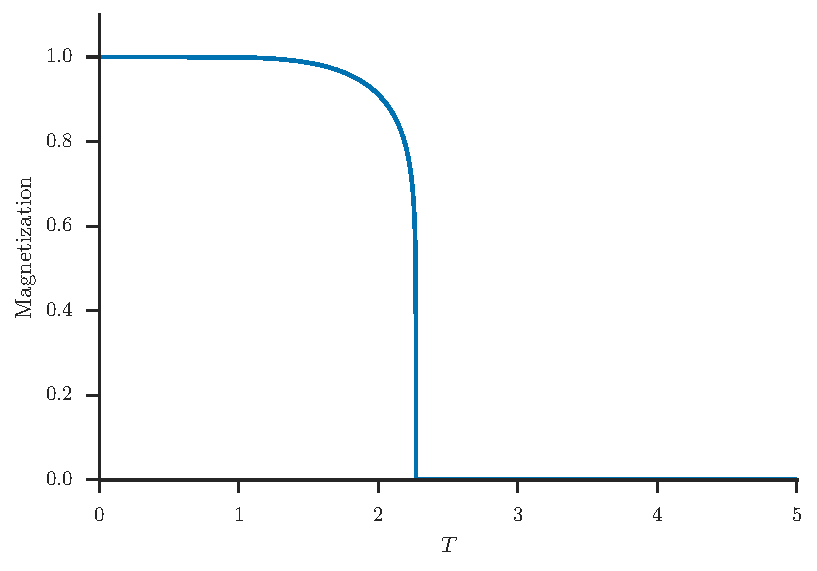
\includegraphics[width=0.66\textwidth]{ising_magnetization}
	\caption{The magnetization of the two-dimensional Ising model. Notice how the magnetization is finite on one side of the phase transition, but zero on the other side.}
	\label{fig:ising_magnetization}
\end{figure}

When we consider phase transitions, we distinguish two different kinds.
The phase transition associated with freezing water is what is called first-order.
As the critical temperature is crossed the water molecules move from a disordered phase into an ordered crystal phase.
As this happens, energy is emmited in the form of latent heat.
This is defined as
\begin{equation}
	\label{eq:latent_heat}
	l = \int_{T_c-}^{T_c+} c(T) \dif T,
\end{equation}
with \(l\) the latent heat and \(c(T)\) the heat capacity of the system.
In first order transition the order parameter is discontinous at \(T_c\).\cite{binney:1992}
In the rest of this work we only consider second-order transitions, for which the latent heat is zero and the order parameter, but not the rate of change of the order parameter is continuous at \(T_c\).

While the latent heat of a transition may be zero, this need not be the case for the heat capacity of the system or other thermodynamic properties such as the magnetic susceptibility.
Often the heat capacity diverces as \(c \propto \abs{T-T_c}^{-\alpha}\).
We call \(\alpha\) a critical exponent.
Because for continuous phase transitions the latent heat has to vanish by definition, \(\alpha\) has to be smaller than 1, because otherwise the integral of \cref{eq:latent_heat} diverges.
No divergence occurs if \(\alpha < 0\).
In the limiting case that \(\alpha = 0\), we can consider the divergence of the specific heat to be logarithmic since
\begin{equation}
	\log(\frac{1}{x}) = \lim_{\alpha \to 0+} \frac{1}{\alpha}\left(x^{-\alpha} - 1\right),
\end{equation}
where \(x = \abs{T - T_c}/T_c\).
Theoretically and experimentally we find that the exponent governing divergence is the same both above and below \(T_c\).\cite{binney:1992}

\subsection{Correlation Functions}
For the systems we would like to consider it is often interesting to quantify how different parts of system relate to each other.
In fact we will see that this correlation proves critical when choosing an appropriate algorithm to numerically study systems around the critical temperature (\cref{sec:critical_slowing_down}).
To quantify the correlations in a system we define the two-point correlation function\cite{binney:1992}, which, to illustrate some properties of the correlation function, we first define for a system of spins:
\begin{equation}
	G^{(2)}(\mathbf{i}, \mathbf{j}) = \langle{\mathbf{s}_i \cdot \mathbf{s}_j}\rangle.
\end{equation}
Here \(\mathbf{i}\) and \(\mathbf{j}\) are the position vectors of the spins at locations \(i\) and \(j\) respectively.
The angle brackets denote thermal averaging.
Because the system is often translationally invariant as well as isotropic, meaning it has no preferred direction, such as in a crystal lattice or in disordered systems, \(G^{(2)}\) often depends only on \(\abs{\mathbf{i} - \mathbf{j}} \)

In the general case the two-point correlation function is defined as
\begin{equation}
	G^{(2)}(r) = \langle \boldsymbol{\phi}(0) \cdot \boldsymbol{\phi}(\mathbf{r}) \rangle,
\end{equation}
where \(\phi\) is the order parameter of the system.
Below \(T_c\) the system is ordered and \(G^{(2)}\) is large for all \(r\).
In the example using spins given above, this means almost all spins are aligned.
A more useful quantity in this case is the connected correlation function
\begin{equation}
	G_c^{(2)} = \langle \boldsymbol{\phi}(0) \cdot \boldsymbol{\phi}(\mathbf{r}) \rangle - \abs{\langle \phi \rangle}^2.
\end{equation}
By subtracting the thermally averaged value of the order parameter from the two-point correlation function, we can ignore the general alignment of the order parameter and only have fluctuations in the order parameter contribute.

When \(T/T_c\) is either large or small \(G_c^{(2)}\) is small.
Precisely at the critical temperature \(G_c^{(2)}\) has the form
\begin{equation}
	G_c^{(2)} \propto \frac{1}{r^{d-2+\eta}},
\end{equation}
with \(d\) the dimensionality of the system and \(\eta\) another critical exponent.
Far away from \(T_c\) \(G_c^{(2)}\) can not be approximated by a power law, but for \(\abs{T-T_c} / T_c \ll 1\) \(G_c^{(2)}\) has the form
\begin{equation}
	G_c^{(2)} \propto \frac{e^{-r/\xi}}{r^{d-2+\eta}}.
\end{equation}
\(\xi\) denotes the correlation length.
Fluctuations of the order parameter up to this length scale are common, but larger fluctuations are exponentially suppressed.
The correlation length diverges as \(T_c\) is approached from above or below, according to
\begin{equation}
	\xi \propto \abs{T-T_c}^{-\nu},
\end{equation}
where \(\nu\) is another critical exponent.

\subsection{Scaling Laws} \label{sec:scaling_laws}
We can define three other critical exponents.
For the magnetic susceptibility we have
\begin{equation}
	\chi \propto \abs{T-T_c}^{-\gamma},
\end{equation}
while for the magnetization of a system we have
\begin{equation}
	\label{eq:magnetization_beta}
	m \propto \abs{T-T_c}^{\beta} \mathrm{\ \ \ \ \ T \to T_c\ from\ below}.
\end{equation}
Finally we can define a critical exponent for the magnetization in a non-zero magnetic field (the previous five critical exponents assumed \(B=0\)).
Precicesly at \(T_c\)
\begin{equation}
	m \propto B^{1/\delta} \mathrm{\ \ \ \ \ B \to 0}.
\end{equation}

These six critical exponents are not independent of each other but are related through scaling laws.
Given these scaling laws only two critical exponents need to be known to determine all others as well.
They are:
\begin{align}
	\alpha + 2\beta +\gamma &= 2\\
	\alpha + \beta(\delta+1) &= 2\\
	(2-\eta)\nu &= \gamma \\
	\nu d &= 2- \alpha,
\end{align}
with \(\nu\) the dimensionalty of the system.\cite{binney:1992,baxter:1989,landau:2015}


\subsection{Universality}
One property of critical phenomena that simplifies their study is the concept of universality.
This is the independence of many thermodynamic properties on the exact details of the hamiltonian of the system.
They will only depend on the dimensionality of the system and symmetries of the Hamiltonian
Consider the hamiltonian
\begin{equation}
	H(s) = H_0(s) + \lambda H_1(s),
\end{equation}
where \(s\) denotes the state of the system, \(H_0\) is a part with a given symmetry, and \(H_1\) does not have that symmetry.
The critical exponents then only depend on \(\lambda\) in that they have one value when \(\lambda=0\) and another when \(\lambda \neq 0\).
This also means that, if both \(H_0\) and \(H_1\) have the same symmetries, then, if \(H_0\) is some simple hamiltonian while \(H_1\) is more complicated, it is possible to obtain the critical exponents of a system using the simple part while stripping the more complicated part.
This may significantly ease the determination of critical exponents when performing simulations.
Different systems with the same critical exponents are said to be in the same universality class.
It is believed (and experimentally established with error) that such diverse systems as carbon dioxide, xenon and the three-dimensional Ising model are in the same universality class.\cite{baxter:1989}

\section{The Two-Dimensional Ising Model} \label{sec:ising_model}

To validate methods to determine critical exponents for systems that are not exactly solvable, a control system that is exactly solved is useful. To that end we study the two-dimensional Ising model in zero-field, first solved exactly in 1944 by Lars Onsager.\cite{onsager:1944}
It describes a square lattice with nearest neighbour interactions, where each lattice point has with it associated a number (which we will refer to as spin) which may either be +1 or -1 and was originally meant as a model for magnets.
The Hamiltonian in zero-field is\cite{mccoy:1973}
\begin{align}
	H = -J_{1} \sum_{j=1}^{\mathcal{M}} \sum_{k=1}^{\mathcal{N}} \sigma_{j,k} \sigma_{j,k+1} - J_{2} \sum_{j=1}^{\mathcal{M}} \sum_{k=1}^{\mathcal{N}} \sigma_{j,k} \sigma_{j+1,k},
\end{align}
with \(\mathcal{M}\) and \(\mathcal{N}\) the extent of the lattice in the \(x\)- and \(y\)-directions respectively and \(J_{1}\) and \(J_{2}\) the interaction strength between neighbours in respectively the \(x\)- and \(y\)-directions.
In the case where the interaction strength in both directions is the same the Hamiltonian becomes\cite{newman:1999}
\begin{align}
	\label{eq:isotropic_hamiltonian}
	H = -J \sum_{\langle ij \rangle} \sigma_{i} \sigma_{j},
\end{align}
where the bracket denotes summation over nearest neighbours.\footnote{Note that naively applying this Hamiltonian to calculate the lattice energy overcounts the energy by a factor of 2 since each bond is counted twice.}
In the ferromagnetic ground state (\(J>0\)) all spins on the lattice are aligned in one of two possible directions (the direction is chosen when the mirror symmetry in the lattice plane is spontaneously broken as the lattice cools).
The Hamiltonian is subject to toroidal boundary conditions in both directions, meaning \(\sigma_{1,k} = \sigma_{\mathcal{M}+1,k}\) and \(\sigma_{j,1} = \sigma_{j,\mathcal{N}+1}\).
We are interested in the thermodynamic properties of the Ising Model.
To that end we define the partition function
\begin{align}
	Z &= \sum_{\sigma = \pm 1} e^{-\beta H} \\
	  &= \sum_{\sigma = \pm 1} \prod_{j=1}^{\mathcal{M}} \prod_{k=1}^{\mathcal{N}} e^{\beta J_1 \sigma_{j,k} \sigma_{j,k+1}} \prod_{j=1}^{\mathcal{M}} \prod_{k=1}^{\mathcal{N}} e^{\beta J_2 \sigma_{j,k} \sigma_{j+1,k}},
\end{align}
with \(\beta=1/k_B T\) and the sum running over every possible orientation of the spins on the lattice. Solving this requires a non-trivial amount of effort and it is best to refer to either Onsager\cite{onsager:1944}, who systemically added one-dimensional Ising models together to create a two dimensional lattice, or Kasteleyn as described in \cite{mccoy:1973}, whose approach considerably simplifies the derivation by reducing it to a combinatorial problem.

The derivation introduces a sign ambiguity in \(Z\) which takes some additional care to resolve, but we can avoid having to deal with this by considering the free energy \(F\) in the thermodynamic limit\footnote{This is the limit in which the number of particles on the lattice tends to infinity.} instead of the partition function
\begin{dgroup*}
	\begin{dmath*}
		F = -\frac{1}{\beta} \lim_{\substack{\mathcal{N} \to \infty \\ \mathcal{M} \to \infty}} \frac{1}{\mathcal{M} \mathcal{N}} \log({Z_{\mathcal{M}, \mathcal{N}}})
	\end{dmath*}
	\begin{dmath}
		= -\frac{1}{\beta} \left[ \log(2) + \frac{1}{2} \frac{1}{(2\pi)^2} \int_{0}^{2\pi} \dif \theta_{1} \int_{0}^{2\pi} \dif \theta_2 \log \bigg(\cosh{(2\beta J_1)} \cosh{(2\beta J_2)} - \sinh{(2\beta J_1)} \cos{(\theta_1)} - \sinh{(2\beta J_2)} \cos{(\theta_2)}\bigg) \right].
	\end{dmath}
\end{dgroup*}

\(F\) is an analytic function of the temperature \(T\), except at one value, which we will call the critical temperature \(T_c\). At this temperature we can define the equality\cite{mccoy:1973}
\begin{align}
	\abs{z_1} &= \frac{1 - \abs{z_2}}{1+ \abs{z_2}}, \text{ with } z_1 = \tanh(2\beta J_1), z_2 = \tanh(2\beta J_2).
\end{align}
Rewriting and squaring this gives
\begin{align}
	\label{eq:ising_z_functions}
	1 - \abs{z_1 z_2} &= \abs{z_1} + \abs{z_2}\rightarrow\\
	\left(1 - z_1^2 \right) \left(1 - z_2^2 \right) &= 4 \abs{z_1 z_2}
\end{align}
Finally, using
\begin{align}
	\frac{1}{2 z_k}\left(1 - z_k^2\right) = \frac{1}{\sinh(2 \beta J_k)}, \text{ with } k \in \{{1, 2}\}
\end{align}
we get the equality
\begin{align}
	1 = \sinh(2\beta J_1) \sinh(2\beta J_2).
\end{align}
In the case where interaction strength in both the \(x\)- and \(y\)-directions is the same (\(\abs{J_1} = \abs{J_2} = J\)) we get an expression for the critical temperature in terms of the bond energy
\begin{align}
	1 &= \sinh(2\beta J) \to \\
	k_B T_c &= \frac{2}{\text{asinh}(1)}J = \frac{2}{\log(1+\sqrt{2})}J \approx 2.269 J
\end{align}
Onsager \cite{onsager:1944} also calculated the values of the free energy, internal energy and entropy at the critical temperature\footnote{We use lowercase letters to denote the thermodynamic properties of a single spin on the lattice and uppercase letters when refering to the entire lattice. Taking as an example the internal energy, \(U/N = u\) with \(N\) the number of spins on the lattice.}:
\begin{align}
	-\frac{f_c}{k_B T} &= \frac{1}{2} \log{2} + \frac{2}{\pi} G \approx 0.929, \\
	u_c &= - \sqrt{2} J \approx - 1.414 J,\\
	\frac{s_c}{k_B} &= \log{(\sqrt{2} e^{2G/\pi})} - \sqrt{2} \frac{J}{k_B T} \approx 0.306
\end{align}
with \(G\) Catalan's constant.\footnote{\(G = 1^{-2} - 3^{-2} + 5^{-2} - 7^{-2} \approx 0.916\)}

\subsection{Thermodynamic Properties of the Two-Dimensional Ising Model}\todo{Check the formula in this part with McCoy, with special attention to factors of two and exponents!}
From the free energy it is relatively simple to determine the specific heat per spin and the internal energy per spin by taking the appropriate derivatives of the free energy\cite{mccoy:1973}. We work with the isotropic case where \(\abs{J_1} = \abs{J_2} = J\) and \(z_1 = z_2 = z = \tanh(\beta J)\), corresponding to \cref{eq:isotropic_hamiltonian}.
Then the expression for the free energy becomes
\begin{dmath}
	F = -\frac{1}{\beta} \left[\log(2\cosh^2(\beta J)) + \log(1+z^2) + \frac{1}{(2\pi)^2} \int_0^{\pi}\dif \theta_1 \int_0^{\pi} \dif \theta_2 \log(1-\frac{1}{2}k \Big\{\cos(\theta_1) + \cos(\theta_2)\Big\})\right],
\end{dmath}
with
\begin{align}
	\label{eq:elliptic_argument}
	k = \frac{4z(1-z^2)}{(1+z^2)^2} = \frac{2\sinh(2\beta J)}{\cosh^2{(2\beta J)}}.
\end{align}
Performing the substitutions \(\omega_1 = \frac{1}{2}(\theta_1 + \theta_2)\) and \(\omega_2 = \frac{1}{2}(\theta_1 - \theta_2)\) and integrating over \(\omega_1\) the free energy becomes
\begin{align}
		F &= -\frac{1}{\beta} \left[\log(2\cosh(2\beta J)) + \frac{1}{\pi^2} \int_0^{\frac{\pi}{2}} \dif \omega_1 \int_0^{\frac{\pi}{2}} \dif \omega_2 \log(1- k \Big\{\cos(\omega_1) + \cos(\omega_2)\Big\})\right]\\
		&= -\frac{1}{\beta} \left[\log(\sqrt{2}\cosh(2\beta J)) + \frac{1}{\pi} \int_0^{\frac{\pi}{2}} \dif \omega \log(1+\left\{1-k^2 \cos^2(\omega)\right\}^{\frac{1}{2}}) \right]
\end{align}

We will take derivatives from this expression to determine expressions for thermodynamic properties. The internal energy per spin is
\begin{align}
	\label{eq:internal_energy}
	u &= \frac{\partial \beta F}{\partial \beta}\\
	&= -2 J \tanh(2\beta J) + k \frac{\dif k}{\dif \beta} \frac{1}{\pi} \int_0^{\frac{\pi}{2}} \dif \omega \frac{\sin^2(\omega)}{\Delta (1+\Delta)}
\end{align}
with
\begin{align}
	\Delta = \left( 1 - k^2 \sin^2(\omega) \right)^{\frac{1}{2}}.
\end{align}

Note that the argument of the integral in \cref{eq:internal_energy} can be rewritten as
\begin{align}
	\frac{\sin^2(\omega)}{\Delta (1+\Delta)} = \frac{(1 - \Delta) \sin^2(\omega)}{\Delta(1-\Delta^2)} = \frac{1}{k^2}\left(\frac{1}{\Delta} - 1\right),
\end{align}
from which it follows that
\begin{align}
	u = - 2 J \tanh(2\beta J) + \frac{1}{\pi} \frac{1}{k} \frac{\dif k}{\dif \beta} \left[ K(k) - \frac{\pi}{2}\right].
\end{align}
Here \(K(k)\) is the complete elliptic integral of the first kind
\begin{align}
	K(k) = \int_0^{\frac{\pi}{2}} \frac{\dif \phi}{\left(1-k^2 \sin^2(\phi)\right)^{\frac{1}{2}}}.
\end{align}
Taking the derivative of \(k\)
\begin{align}
	\label{eq:k_derivative}
	\frac{1}{k}\frac{\dif k}{\dif \beta} = \frac{2 J}{\tanh(2\beta J)} (1 - 2\tanh^2(2 \beta J)),
\end{align}
the internal energy per spin becomes (see \cref{fig:ising_internal_energy}) for a plot)
\begin{align}
	\label{eq:ising_internal_energy}
	u = \frac{-J}{\tanh(2\beta J)} \left[1 + \frac{2}{\pi} \left\{2 \tanh^2(2\beta J) -1 \right\} K(k) \right].
\end{align}

For the specific heat per spin we take the derivative of the internal energy per spin with respect to the temperature
\begin{dgroup}
	\begin{dmath}
		c = \frac{\partial u}{\partial T} \hiderel{=} \frac{-1}{k_B T^2}\frac{\partial u}{\partial \beta}
	\end{dmath}
	\begin{dmath}
		= \frac{J}{k_B T^2} \left[\frac{-2J}{\cosh^2(2\beta J)}\left\{ 1 + \frac{2}{\pi} \left(2 \tanh^2(2\beta J) -1 \right) K(k) \right\}\right]
		+ \frac{16}{\pi} \frac{J}{\tanh^2{2\beta J}} K(k) + {\frac{2}{\pi}\frac{\left(2 \tanh^2(2\beta J) -1 \right)}{\tanh(2\beta J)}\\
		 \frac{\dif k}{\dif \beta} \frac{\dif K(k)}{\dif k}}.
	\end{dmath}
\end{dgroup}
For the derivative of the elliptic integral we use the identity\cite{mccoy:1973}
\begin{align}
	\frac{\dif K(k)}{\dif k} = \frac{1}{k k^{'2}} \left[E(k) - k^{'2} K(k) \right],
\end{align}
where \(E(k)\) is the complete elliptic integral of the second kind
\begin{align}
	\label{eq:elliptic_identity}
	E(k) = \int_0^{\frac{\pi}{2}} \dif \phi \left(1-k^2 \sin^2(\phi)\right)^{\frac{1}{2}},
\end{align}
and \(k^{'2} = 1 - k^2\).
Using \cref{eq:k_derivative} and \cref{eq:elliptic_identity} the expression for the specific heat per spin becomes (see \cref{fig:ising_internal_energy} for a plot)
\begin{align}
	\label{eq:ising_heat_capacity}
	c = k_B \left[ \frac{\beta J}{\tanh(2\beta J)} \right]^{2} \frac{2}{\pi} \left[ 2 K(k) -2 E(k) - \left(1 - k' \right) \left\{ \frac{\pi}{2} + k' K(k) \right\}\right].
\end{align}

\begin{figure}[h]
	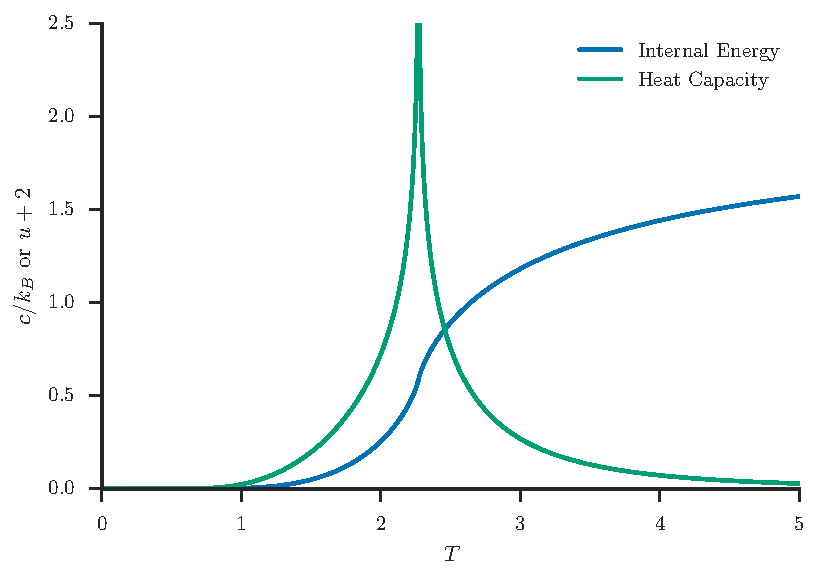
\includegraphics[width=0.66\textwidth]{ising_internal_energy.pdf}
	\caption{The internal energy per site and the specific heat per site of the two-dimensional Ising model in zero-field. Notice the divergence of the specfic heat around \(T=T_c \approx 2.269\), which is cutoff in this graph due to the limited resolution.}
	\label{fig:ising_internal_energy}
\end{figure}

\subsection{The Ising Model around \(T_c\)}

Given that we would like to know how the Ising model behaves around \(T_c\), we need to expand the expressions for the internal energy and the heat capacity around this temperature.
When \(T \approx T_c\) the argument \(k\) as defined in \cref{eq:elliptic_argument} of the elliptic integrals in the definitions \cref{eq:ising_internal_energy} and \cref{eq:ising_heat_capacity} becomes approximatly 1. More precisily
\begin{align}
	k &\approx 1 - 4 \beta_c^2 J^2 (\frac{T}{T_c} - 1)^2, \\
	k^' &\approx 2 \sqrt{2} \beta_c J (\frac{T}{T_c} - 1)
\end{align}
with \(\beta_c = \frac{1}{k_B T_c}\).
It is obvious that for \(k = 1\) \(E(k) = 1\) whereas \(K(1)\) diverges since the integral becomes
\begin{align}
	\int_0^{\frac{\pi}{2}}\frac{1}{\cos{\theta}} \dif \theta \to \infty
\end{align}
Nevertheless an approximation around \(k = 1\) yields \(K(k) \approx \log(\frac{4}{k^'})\).

At \(T_c\) the internal energy per spin \(u\) does not diverge and has the value
\begin{align}
	u(T_c) = \frac{-J}{\tanh(2\beta_c J)} = -\sqrt{2}J.
\end{align}
The heat capacity per spin \(c\) does diverge. Using the previous expansions
\begin{align}
	\frac{c(T)}{k_B} &\approx \frac{8}{\pi} \left(\beta_c J\right)^2 \left[\log(\frac{4}{k^'})\right] \\
	&= \frac{2}{\pi} \log(1 + \sqrt{2})^2 \left[-\log(\frac{T}{T_c} - 1) - 1 - \frac{\pi}{4} - \log(\frac{\sqrt{2}}{4} \log(1+\sqrt{2}))\right]
\end{align}
and we see \(c\) diverging logarithmically as \(T \to T_c\).
This means that the critical exponents \(\alpha = 0\) for the two-dimensional Ising model.
When Onsager first solved the model, it also highlighted the first instance of universality.
Onsager considered the general case where the interaction energy in the \(x\)- and \(y\)-directions differed, but the logarithmic divergence depended only on the critical temperature, and not on the ratio \(J_1 \ J_2\).\cite{baxter:1989}
Note that the sharp phase transition as described here only occurs when the lattice is of infinite extent.
When we do not operate in the thermodynamic limit the partition function of the Ising model is analytic for all \(T\) and has a maximum but no divergence at \(T_c\).\cite{onsager:1944}


\subsection{Magnetization of the Ising Model} \label{sec:ising_magnetization}

Onsager also calculated the magnetization of the Ising model.
On the square lattice with \(T < T_c\) and \(J_1, J_2 > 0\) the magnetization squared is equal to the spin-spin correlation function
\todo{Is this m or M?}
\begin{equation}
	M^2 = \lim_{N \to \infty} \langle \sigma_{00} \sigma_{0,N} \rangle = \lim{N \to \infty} \langle \sigma_{00} \sigma_{N, N} \rangle.
\end{equation}
Determining the correlation function is non-trivial, but the result is\todo{Check the exponents with McCoy}
\begin{equation}
	M^2 = \lim_{N \to \infty} \langle \sigma_{00} \sigma_{0,N} \rangle = \left[ \frac{(1-\alpha_1^2)(1-\alpha_2^2)}{(1-\alpha_1 \alpha_2)^2}, \right]^{1/4}
\end{equation}
with
\begin{equation}
	\alpha_1 = \frac{z_1(1-\abs{z_2})}{1+\abs{z_2}}, \alpha_2 = \frac{1}{z_1}\frac{1-\abs{z_2}}{1+\abs{z_2}},
\end{equation}
where we use \(z_1\) and \(z_2\) as defined in \cref{eq:ising_z_functions}.
The magnetization is then (see \cref{fig:ising_magnetization} for a plot)
\begin{equation}
	M = \left[1 - \left\{\sinh(2\beta J_1)\sinh(2 \beta J_2)\right\}^{-2} \right]^{1/4}.
\end{equation}
When we approach the critical temperature from below we can expand around \(T_c\) and get
\begin{equation}
	M \propto \left[4\beta_c\left\{\frac{J_1}{\tanh(2\beta J_1)} + \frac{J_2}{\tanh(2\beta J_2)}\right\} \left\{1-\frac{T}{T_c}\right\}\right]^{1/8}.
\end{equation}
Comparing with \cref{eq:magnetization_beta} we see that \(\beta = 1/8\).\cite{wu:1982}

Finally the magnetic susceptibility can be shown to diverge as \(\chi \propto \abs{T - T_c}^{-7/4}\), giving \(\gamma = 7/4\).
With the earlier result \(\alpha=0\), we can use the scaling laws (\cref{sec:scaling_laws}) to determine that \(\delta = 15\), \(\eta = 1/4\) and \(\nu = 1\).\cite{binney:1992}

\section{The Potts Model}
The Potts model was first defined by Potts in 1953 as a generalization of the Ising model on the suggestion of Domb, his supervisor.\cite{potts:1952}
Domb suggested that that to generalize, we can consider the spins of the model to be confined to a plane, with each spin pointing in one of \(q\) equally spaced directions, separated by an angle \(\theta_n = 2\pi n /q\), with \(n = 0, 1, \ldots q - 1\).
The nearest neighbour interaction depend only on the angle between those neighbours.
The hamiltonian for this system is
\begin{equation}
	H = - \sum_{\langle i, j \rangle} J(\theta_{ij}),
\end{equation}
with \(J(\theta)\) a \(2\pi\)-peridic function and \(\theta_{ij} = \theta_i - \theta_j\) the angle between two spins.
Domb suggested to use \(J(\theta_{ij}) = - \epsilon_1\cos(\theta_{ij})\).
This is now known as the planar Potts model.\cite{wu:1982}

Making use of a duality relation which showed that the partition function at a low temperature \(T\) was equal to that at a high temperature \(T^*\), (\(Z(T)=Z(T^*)\)) Potts found the critical temperature for \(q=2, 3, 4\), by assuming that there is exactly one temperature for which \(T=T^*\).
This method was first used by Kramers and Wannier in 1941\cite{kramers:1941}, to determine the critical temperature of the two-dimensional Ising model three years before Onsager's exact solution.

Potts also gave a formula for the critical temperature of a system with a different interaction strength: \(J(\theta_{ij}) = -\epsilon_2 \delta(\sigma_i, \sigma_j)\), where \(\delta\) is the Kronecker delta.
For this system he established that for all \(q\) the transition ocurres at\cite{potts:1952}
\begin{equation}
	\frac{x_0}{x_1} = 1 + \sqrt{q},
\end{equation}
with
\begin{align}
	x_0 &= e^{-J_0 / k_B T} \mathrm{\ \ \ \ \ for\ spins\ in\ like\ orientations,}\\
	x_1 & = e^{-J_1 / k_B T} \mathrm{\ \ \ \ \ for\ spins\ in\ unlike\ orientations}.
\end{align}
For \(q=3\) we find that the critical temperature is \(T_c=\frac{1}{\log(1+\sqrt{3})} \approx 0.995\).\cite{fan:2007}
We call this system the standard Potts model.
Throughout the rest of this thesis we will mainly consider this model and will simply refer to it as the Potts model.
The planar and standard Potts models are related for \(q = 2\) by \(\epsilon_2 = 2 \epsilon_1\) and for \(q=3\) by \(\epsilon_2 = \frac{3}{2} \epsilon_1\).
For the Potts model in two dimensions the transition at the critical point is first-order for \(q > 4\) and second-order for \(q \leq 4\).\cite{wu:1982,baxter:1973}
Potts found that an earlier result by Ashkin and Teller for the discontinuities of the energy and specific heat\cite{ashkin:1943}, \(\Delta E, \Delta C\), could be generalized to show the relationship between those quantities:
\begin{equation}
	\sqrt{q}T \Delta E = \log(\frac{x_0}{x_1}) \Delta E.
\end{equation}
Therefore transitions with a continuos energy exclude the possibility of a discontinuous heat capacity.
This does however not mean that the specific heat needs to be finite at \(T_c\).


At the critical temperature the internal energy is\cite{baxter:1989,binder:1981a}
\begin{equation}
	u_{\mathrm{average}} = -\left(1+\frac{1}{\sqrt{q}}\right)J,
\end{equation}
with
\begin{equation}
	u_{\mathrm{average}} = \frac{1}{2} (u_c^+ + u_c^-),
\end{equation}
where \(u_c^+ = \lim_{T \to T_c^+} \langle u \rangle\) and for a second order transition \(u_c^+ = u_c^-\).
For \(q=3\) (a second order transition) \(u_{\mathrm{average}} = -(1+\frac{1}{\sqrt{3}})J \approx - 1.577 J\).

To properly define when the phase transition occurs we define the order parameter, which here is the magnetization, as
\begin{equation}
	m = \frac{1}{N}\abs{\sum_i^N e^{i2\pi n_i / q}},
\end{equation}
with the sum running over every site of the lattice, \(N\) being the number of sites and \(n_i\) being the state of the spin at site \(i\).
This is based on the definition of the \(q\)-state Potts model as consisting of equally spaced vectors.
It has the desired properties of being 1 when all spins on the lattice point in the same direction and being 0 when the spins are equally distributed over the possible states.

The Potts model has not been solved exactly, thus we do not know the exact values of the critical exponents.
There are however other systems in the same universality class as the Potts model.
For \(q=2\) the model reduces to the Ising model and associated exponents (\cref{sec:ising_magnetization}).
For \(q=3\) the model is conjectured to be equal to absorbed monolayers (two-dimensional model), a system that can be probed experimentally and gives \(\alpha = 0.36\)\cite{binder:1981a}.
It is also suspected that the hard hexagon model (a two-dimensional lattice model describing a gas of non-overlapping spheres, placed on a triangular lattice so no two molecules are adjacent) is in this universality class.
This model is exactly solved and has the critical exponents\cite{baxter:1989,wu:1982}
\begin{equation} \label{eq:potts_critical_exponents}
	\alpha = \frac{1}{3},\ \ \beta = \frac{1}{9},\ \ \delta = 14,\ \ \nu = \frac{5}{6},\ \ \gamma = \frac{13}{9},\ \ \eta = \frac{4}{15}.
\end{equation}

While no exact solution exists, Den Nijs has put forth conjectures for the values of the exponents.\cite{nijs:1979}
We have
\begin{equation}
	2 - \alpha = \frac{1}{y_t} ,\ \ \ 1 + \frac{1}{\delta} = \frac{2}{y_h},
\end{equation}
with the thermal and magnetic exponents:
\begin{equation}
	y_t = \frac{3(1-u)}{2-u},\ \ \ y_h = \frac{(3-u)(5-u)}{4(2-u)}.
\end{equation}
For \(q \leq 4\)\cite{wu:1982}
\begin{equation}
	0 \leq u = \frac{2}{\pi} \arccos(\frac{\sqrt{q}}{2}) \leq 1.
\end{equation}
The critical exponents then become\cite{wu:1982, baxter:1989}:
\begin{equation}
	\begin{aligned}[c]
		\alpha &= \frac{2(1-2u)}{3(1-u)}, \\
		\beta &= \frac{1}{12}(1 + u), \\
		\gamma &= \frac{u^2 -4u +7}{6(1+u)}, \\
	\end{aligned}
	\ \ \
	\begin{aligned}[c]
		\delta &= \frac{(3-u)(5-u)}{1-u}, \\
		\nu &= \frac{2-u}{3(1-u)}, \\
		\eta &= \frac{1-u^2}{2(2-u)}.
	\end{aligned}
\end{equation}
For \(q=3\), \(u=1/3\), and these equations reproduce \cref{eq:potts_critical_exponents}.


\chapter{Simulating Lattice Models}

\section{Markov Processes and Monte Carlo Methods}
While some success is to be had by using analytical methods to study lattice models and their critical exponents, often the partition function can not exactly be determined.
At that point we can use computer simulation of the models in question to study phase transitions, while having the exactly solved models as a benchmark for these simulations.

We are almost always interested in the value of a thermal average of a quantity:
\begin{equation}
	\langle X \rangle = \sum_{\alpha}X_{\alpha}p_{\alpha},
\end{equation}
with \(\langle X \rangle\) a thermal average, the sum running over all configurations, each labeled by \(\alpha\), and \(p_{\alpha}\) the Gibbs probability of state \(\alpha\) in equilibrium\cite{binney:1992}:
\begin{equation}
	p_{\alpha} = \frac{e^{-\beta E_{\alpha}}}{\sum_{\alpha}e^{-\beta E_{\alpha}}}.
\end{equation}
While for small lattices (e.g. 3 by 3) the number of states is tractable (this number scales as \(2^{N}\) for the Ising model and \(q^{N}\) for the Potts model), for larger lattices the sum can no longer be performed numerically and some clever way has to be found to sample only important states.
% - sampling and importance sampling
% - briefly mention the origins of Monte Carlo name and Los Alamos

\subsection{Ergodicity and Detailed Balance}

\section{The Metropolis Algorithm}
The Metropolis algorithm, first published by Metropolis \textit{et al.} in 1953 \cite{metropolis:1953}, is a simple algorithm that was first used by its creators to study the dynamics of continuously displaceable hard spheres.
The algorithm is as follows\cite{binney:1992}:
\begin{enumerate}
	\item Choose a random site on the lattice.
	\item Flip the spin on this location and calculate the change in energy \(\Delta E\) associated with this spin-flip.
	\item Calculate the probability of accepting this move:
	\begin{equation}
		A =
		\begin{cases}
			e^{-\beta \Delta E}\ \ \ &\Delta E > 0 \\
			1 \ \ \ &\Delta E \leq 0
		\end{cases}
	\end{equation}
	\item Generate a random variable \(r\) in the interval \(\left[0, 1\right)\).
	\item Accept the move if \(r \leq A\). Otherwise leave the lattice as it was.
\end{enumerate}
The spin flip may also happen to a non-random spin simply by iterating over the rows and columns of the lattice. When studying only equilibrium dynamics, the two approaches are identical.\cite{landau:2015}


% - discuss boundary conditions
% - initial state


\subsection{Critical Slowing Down} \label{sec:critical_slowing_down}
% - correlation times
% - dynamic exponents
% - dynamic universality

\section{The Wolff Algorithm}
The Wolff algorithm goes as follows:
\begin{enumerate}
	\item Choose a random site on the lattice \(i\)
	\item \label{item:wolff_step_two} Look at the neighbours of \(i\). If a neighbour \(j\) has the same spin as \(i\), add it to the cluster with probability \(P = 1 - e^{-2\beta J}\).
	\item Repeat step \ref{item:wolff_step_two} for spin \(j\) until no more spin can be added to the cluster.
	\item Flip the entire cluster.
\end{enumerate}
If a spin was considered during a previous step but not added to the cluster, this spin may be reconsidered for future steps.\cite{newman:1999}
% - mean cluster sizes
\begin{figure}[h]
	\centering
	\includegraphics[width=\textwidth]{20160530161259_Mean_Cluster_Size_as_Fraction_of_Lattice.pdf}
	\caption{The mean size as a fraction of the lattice of clusters generated with the Wolff method. During the simulation the temperature varied from 2 to 3 in steps of 0.1. The errorbars are too small to see.}
\end{figure}

\section{Generalizing Algorithms to the Potts Model}

\section{Optimizations}
When working in a programming language that represents data in continuous blocks of memory such as C, helical boundary condition may improve performance.
% - obvious optimizations for E and m
% - caching exponents

\section{Systemic errors}


\chapter{Analysis of Monte Carlo Simulations}
\section{Statistics}
\subsection{Binning}
\subsection{Bootstrap and Jackknife}
% Define chi, c here
\section{The Binder Cumulant}
Given these statistically independent measurements, one thing we may like to find is the critical temperature.
Unfortunately we can not determine this simply by looking at the order parameter of a system and when it becomes zero, because the finite size of the simulated lattices precludes a sharp phase transition.
We can however define the Binder cumulant\cite{binder:1981b}
\begin{equation}
	U_4 = 1 - \frac{\langle m^4 \rangle}{3 \langle m^2 \rangle^2},
\end{equation}
which for \(L \to \infty\) becomes \(2/3\) for \((T \to 0)\) and 0 for \(T \to \infty\).\cite{landau:2015}
At the critical temperature \(U_4\) has the same value independent of the lattice size.
Therefore the critical temperature can be found by plotting the binder cumulant for different lattice sizes and looking for the intersection (as seen in \cref{fig:ising_binder_cumulant}).
\begin{figure}[h]
	\includegraphics[width=\textwidth]{20160530161301_Binder_Cumulant.pdf}
	\caption{The Binder cumulant for the Ising model at three different lattice sizes. The critical point occurs at approximately \(T = 2.26\). The values were acquired by simulation the lattice using the Wolff algorithm and running 65536 steps after equilibration. The temperature was varied from 2.169 to 2.369 in steps of 0.01. The errorbars are too small to see in this plot.}
	\label{fig:ising_binder_cumulant}
\end{figure}

% Finding the intersection
\section{Finite Size Scaling}
% - Data collapse using chi-square fitting
% - Log-Log plots to find Ratios

\chapter{Results}
The Binder cumulant intersections were found by\todo{Explain}
This was also used to find the error
% - Results for both Ising and Potts
\begin{center}
	\begin{tabular}{l c c c c c c}
		& \(\alpha\) & \(\beta\) & \(\gamma\) & \(\eta\) & \(\nu\) & \(\delta\) \\\hline
		Blöte (1981)\cite{blote:1981} & & \\
		Fan (2007)\cite{fan:2007} & & \\
		Ghamei (2001)\cite{ghaemi:2001} & & \\
		Hu (1980)\cite{hu:1980} & & \\
		Straley (1973)\cite{straley:1973} & & \\
	\end{tabular}
\end{center}

\chapter{Conclusions}

\section{Further Work}
% - More attention to autocorrelation
% - Better definition for the order parameter
% - Measure entropy
% - go to q=4, 5 and try to determine that the transition is first order
% - Analysis using renormalization group methods



% Set style to abbrv to get Vancouver style citations.
\bibliographystyle{abbrv}
\bibliography{bachelor-thesis}

\end{document}
